\section{Correlation and results}
As has been discussed in last section, different characteristic parameters are investigated throughout the whole runs. Except few cases such as long period of spill (see figure \ref{fig:EveN_spill_abnormal}) or double peaks from recoil proton (see figure \ref{fig:Recoil_proton_double_peak}), most of the abnormalities can be depicted by FWHM value of total invariant mass distribution (shown in figure \ref{fig:Total_mass_FWHM}). To decipher the cause behind all these phenomenon, correlations between the abnormalities of different parameters are inquired.
\subsection{Correlation of abnormalities}
The most two obvious parameters that can be correlated to the abnormality of total invariant mass distribution should be recoil proton and photon number captured by both ECALS.
\subsubsection{Correlation with recoil proton}
The angular distribution of recoil proton is directly related to the scattering process. If spectrum and constitution of incoming particle beam are same for each run, the mass of unknown intermediate state $X$ can be reflected by the recoil proton due to four-momentum conservation. As is shown in subsection \ref{subsec:recoil_proton}, the width at lower half of angular distribution could be really large for abnormal runs. To establish the correlation, the value of width for recoil proton can plotted with the value of FWHM of invariant mass distribution for each run (see figure \ref{fig:Total_mass_recoil_proton}). At first sight, strong correlations appear for the run number 69816, 70650, 70654. When there is an increase on FWHM value, there is also an increase on the width from recoil proton. On the other hand, there are also some abnormal runs which are not correlated, such as run number 69811 and range 70223 $\sim$ 70240.
\begin{figure*}[!h]
	\centering
	\vspace{2cm}
	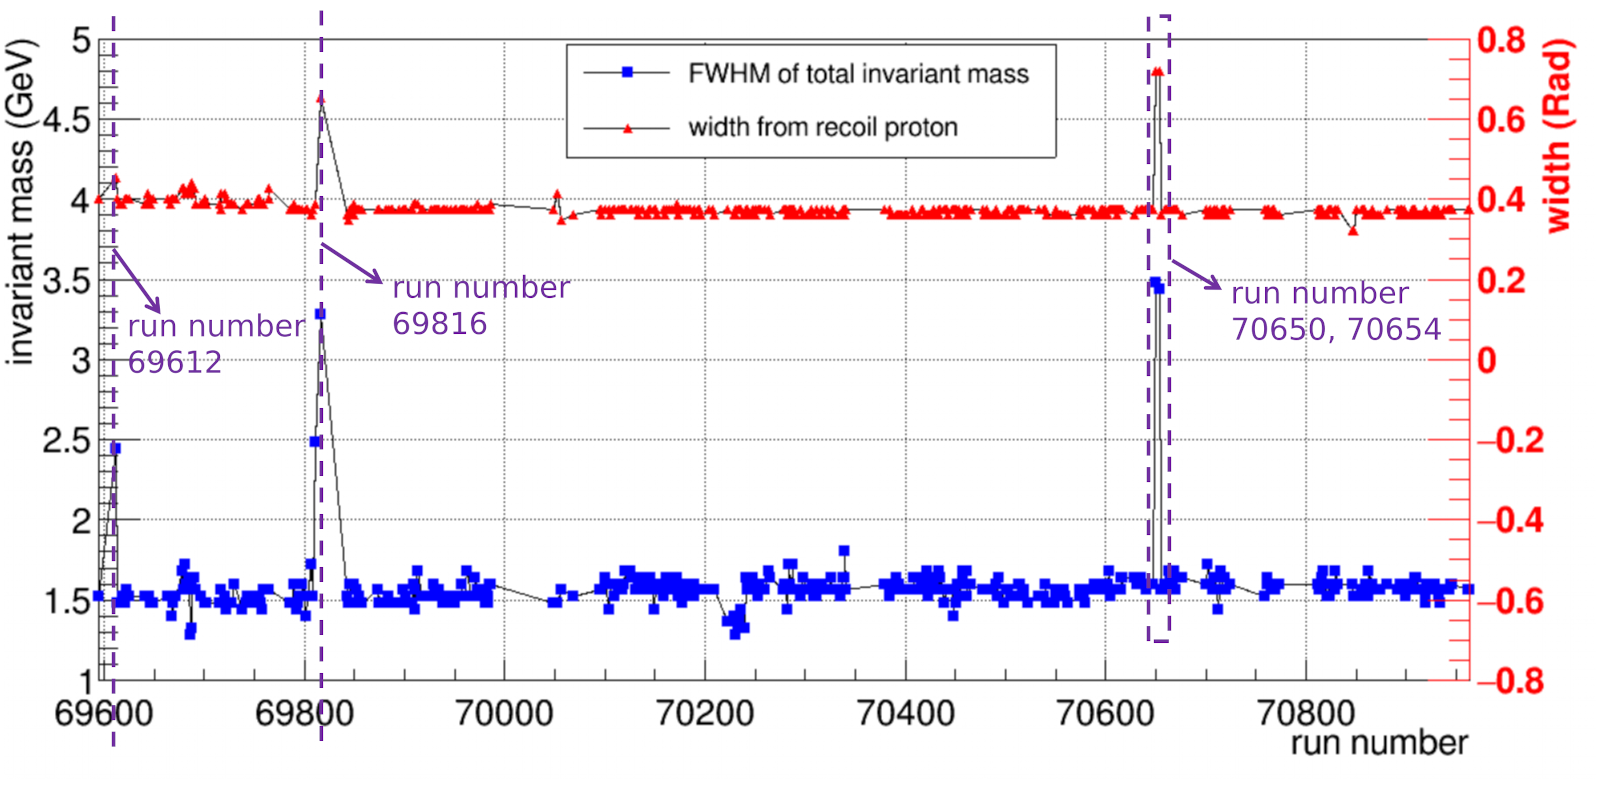
\includegraphics[width=\textwidth]{Total_mass_recoil_proton}
	\caption{Histogram of invariant total mass distribution. The colors inside the histogram represent number of events corresponding to the run number and invariant mass. To better compare and conceive the structure of distribution between runs visually, the maximal value of each distribution is normalized to 1000. In the red dashed rectangles, it can be seen that the red strokes are much longer than the normal runs.}
	\label{fig:Total_mass_recoil_proton}
	\vspace{2 cm}
	
	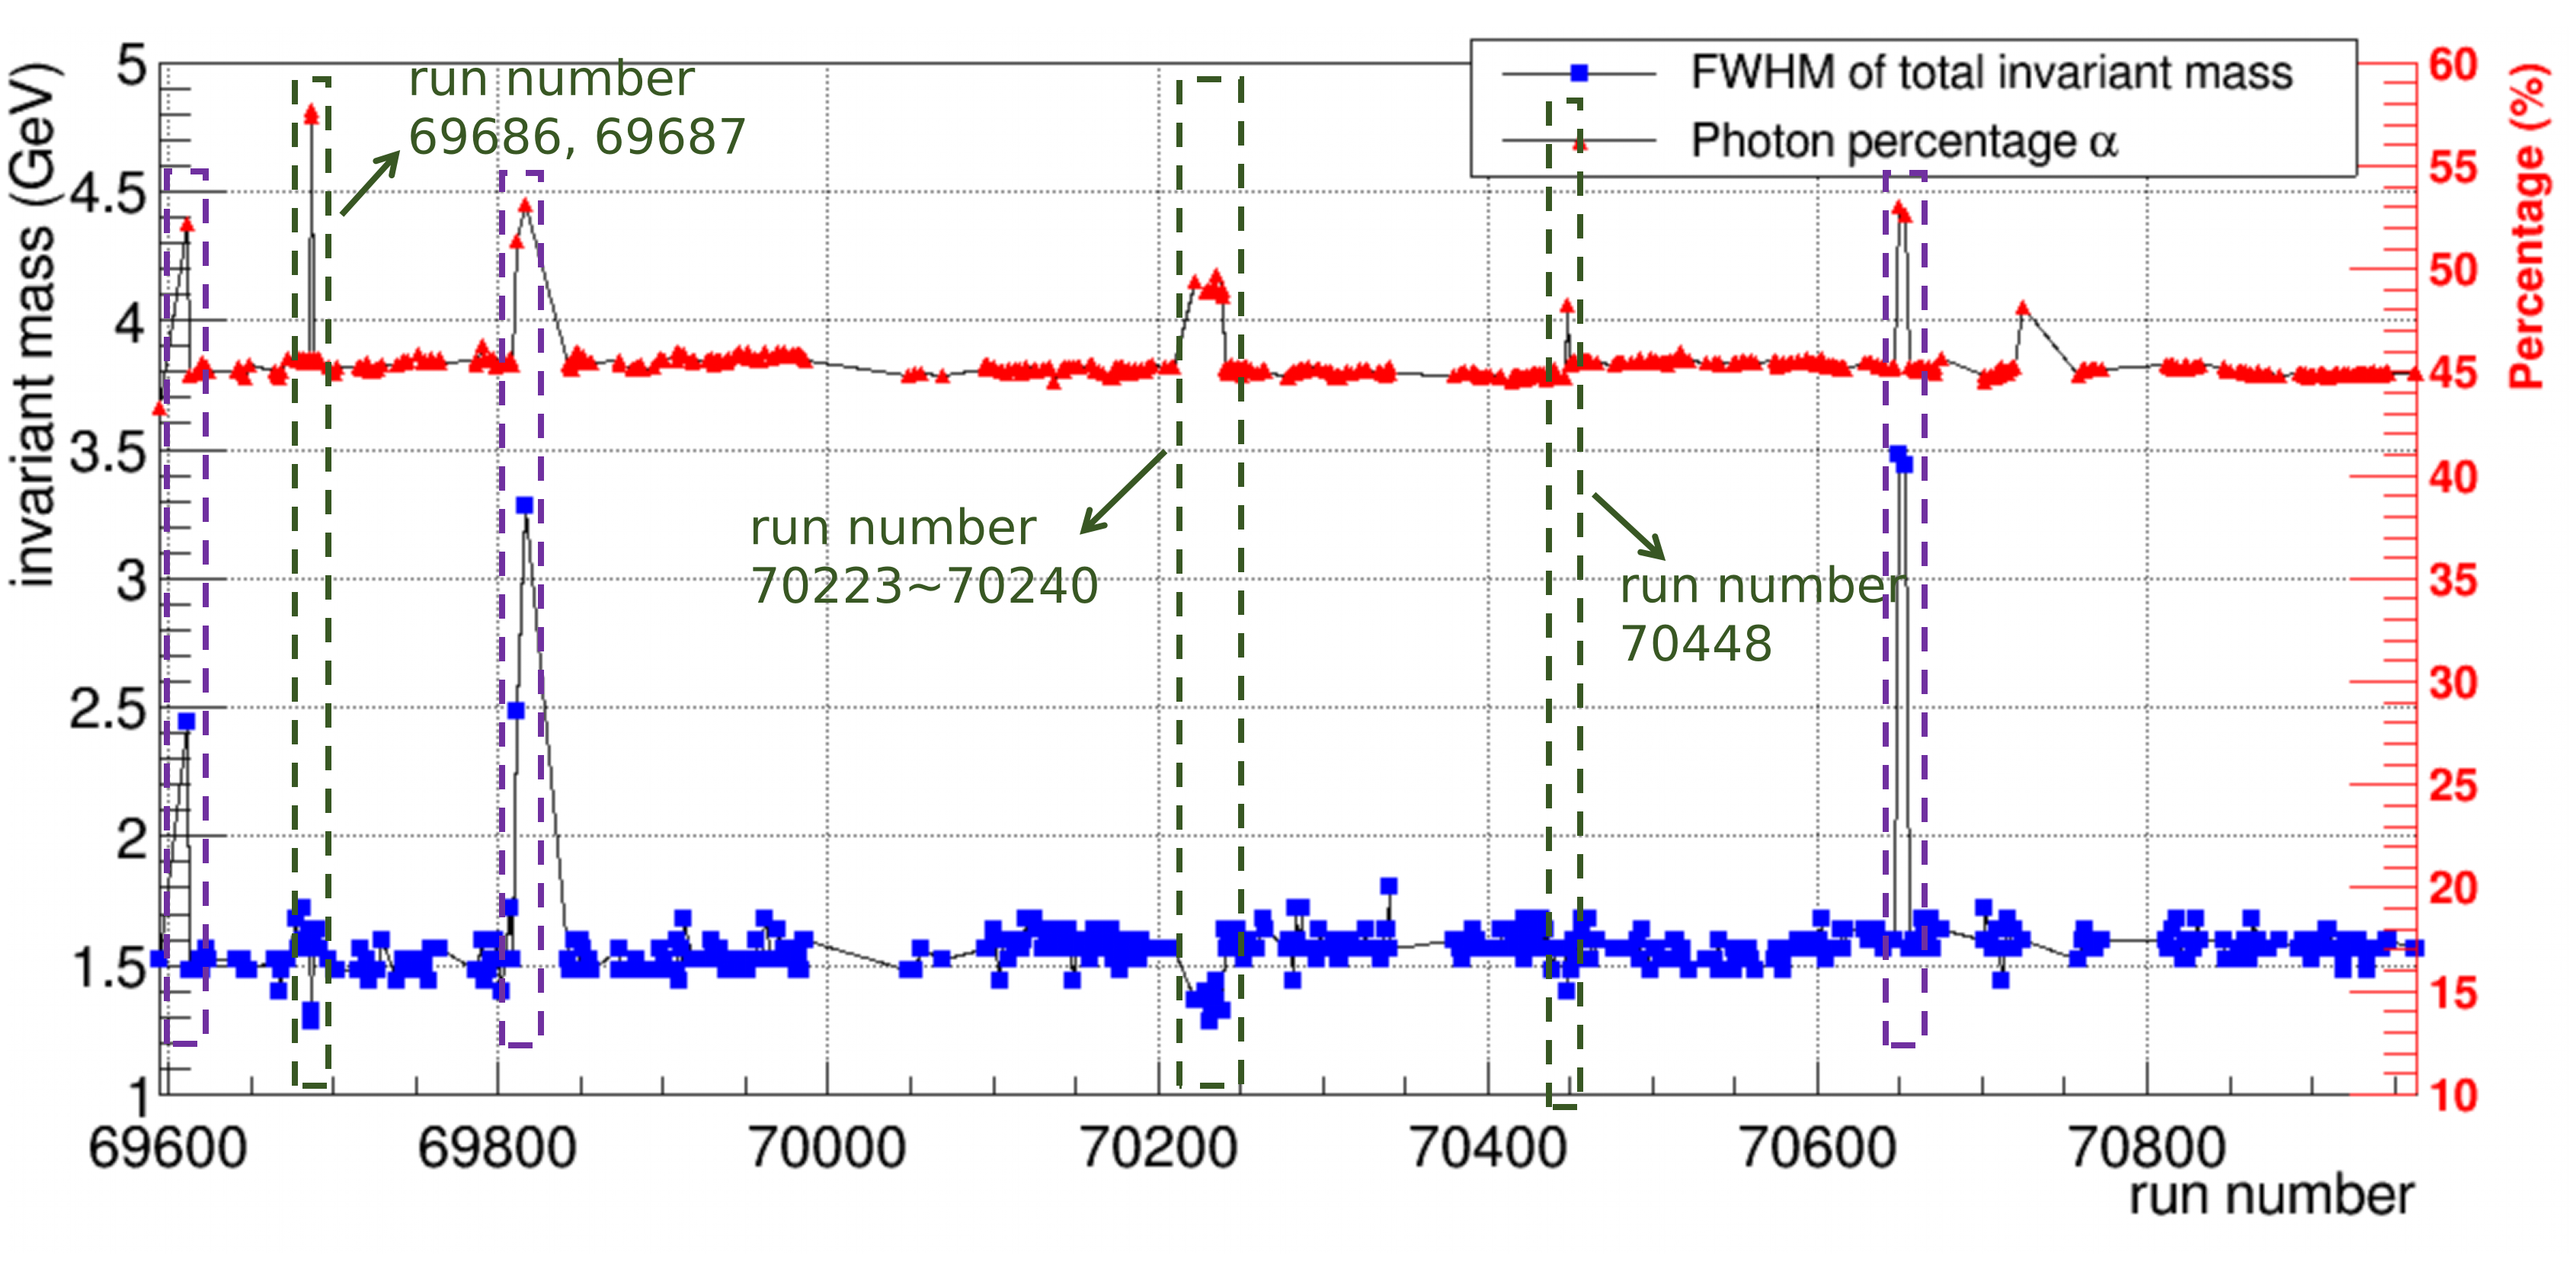
\includegraphics[width=\textwidth]{Total_mass_ECAL}
	\caption{Value of full width at half maximum of total invariant distribution for each run. Typical value of FWHM for normal run is around \SI{1.5}{\giga\electronvolt}.There are several outliners that have much bigger FWHM value than the general one. Also there is a range of runs 70223 $\sim$ 70240 that have slight smaller value of FWHM. }
	\label{fig:Total_mass_ECAL}
	\vspace{3cm}
\end{figure*}
\subsubsection{Correlation with ECALs}
Comparing abnormal runs in figure \ref{fig:Total_mass_FWHM} and figure \ref{fig:Three_pion_mass_Graph}, one can easily notice that most of abnormal runs in total invariant mass distribution fail to show abnormality in invariant mass distribution of three pions.
\subsection{Summary of abnormal runs}
\begin{table}[!h]
	\begin{tabular}{|p{0.1\textwidth}|p{0.15\textwidth}|p{0.2\textwidth}|}
		\hline
		RunNumber        & Abnormality                                      & Log book/comments                 \\ \hline \hline
		70195             & Disorder of spill time                                    & Good                              \\ \hline \hline
		69811             & Three pion mass                                           & Magnets were ramped up during run \\ \hline \hline
		70054             & Double peaks for recoiled proton                          & Errors appeared for SrcID         \\ \hline \hline
		69612             & \multirow{4}{0.15\textwidth}{Recoiled proton angular distribution}     & N/A                               \\ \cline{1-1} \cline{3-3} 
		69816             &                                                           & No sandwich veto                  \\ \cline{1-1} \cline{3-3} 
		70650             &                                                           & Special run to test sandwich veto \\ \cline{1-1} \cline{3-3} 
		70654             &                                                           & No sandwich veto                  \\ \hline \hline
		\parbox[c]{\hsize} {69696}             & \multirow{4}{0.15\textwidth}{Decrease of number of photons from ECAL2} & Detector test                     \\ \cline{1-1} \cline{3-3} 
		69687             &                                                           & Light trigger problems            \\ \cline{1-1} \cline{3-3} 
		70223 $\sim$70240 &                                                           & High voltage trip on ECAL2        \\ \cline{1-1} \cline{3-3} 
		70448             &                                                           & Low intensity beam                \\ \hline
	\end{tabular}
\end{table}